%╔════════════════════════════╗
%║	  Szablon dostosował	  ║
%║	mgr inż. Dawid Kotlarski  ║
%║		  08.10.2022		  ║
%╚════════════════════════════╝
\documentclass[12pt,twoside,a4paper,openany]{article}

    % ------------------------------------------------------------------------
% PAKIETY
% ------------------------------------------------------------------------

%różne pakiety matematyczne, warto przejrzeć dokumentację, muszą być powyżej ustawień językowych.
\usepackage{mathrsfs}   %Różne symbole matematyczne opisane w katalogu ~\doc\latex\comprehensive. Zamienia \mathcal{L} ze zwykłego L na L-transformatę.
\usepackage{eucal}      %Różne symbole matematyczne.
\usepackage{amssymb}    %Różne symbole matematyczne.
\usepackage{amsmath}    %Dodatkowe funkcje matematyczne, np. polecenie \dfac{}{} skladajace ulamek w trybie wystawionym (porównaj $\dfrac{1}{2}$, a $\frac{1}{2}$).

%język polski i klawiatura
\usepackage[polish]{babel}
%\usepackage{qtimes} % czcionka Times new Roman
\usepackage[OT4]{polski}
%\usepackage[cp1250]{inputenc}                       %Strona kodowa polskich znaków.

%obsługa pdf'a
\usepackage[pdftex,usenames,dvipsnames]{color}      %Obsługa kolorów. Opcje usenames i dvipsnames wprowadzają dodatkowe nazwy kolorow.
\usepackage[pdftex,pagebackref=false,draft=false,pdfpagelabels=false,colorlinks=true,urlcolor=blue,linkcolor=black,citecolor=green,pdfstartview=FitH,pdfstartpage=1,pdfpagemode=UseOutlines,bookmarks=true,bookmarksopen=true,bookmarksopenlevel=2,bookmarksnumbered=true,pdfauthor={Dawid Kotlarski},pdftitle={Praca Inznierska},pdfsubject={},pdfkeywords={transient recovery voltage trv},unicode=true]{hyperref}   %Opcja pagebackref=true dotyczy bibliografii: pokazuje w spisie literatury numery stron, na których odwołano się do danej pozycji.

%bibliografia
%\usepackage[numbers,sort&compress]{natbib}  %Porządkuje zawartość odnośników do literatury, np. [2-4,6]. Musi być pod pdf'em, a styl bibliogfafii musi mieć nazwę z dodatkiem 'nat', np. \bibliographystyle{unsrtnat} (w kolejności cytowania).
\usepackage[
backend=biber,
style=numeric,
sorting=none
]{biblatex}
\addbibresource{bibliografia.bib}
\usepackage{hypernat}                       %Potrzebna pakietowi natbib do wspolpracy z pakietem hyperref (wazna kolejnosc: 1. hyperref, 2. natbib, 3. hypernat).

%grafika i geometria strony
\usepackage{extsizes}           %Dostepne inne rozmiary czcionek, np. 14 w poleceniu: \documentclass[14pt]{article}.
\usepackage[final]{graphicx}
\usepackage[a4paper,left=3.5cm,right=2.5cm,top=2.5cm,bottom=2.5cm]{geometry}

%strona tytułowa
\usepackage{strona_tytulowa}

%inne
\usepackage[hide]{todo}                     %Wprowadza polecenie \todo{treść}. Opcje pakietu: hide/show. Polecenie \todos ma byc na koncu dokumentu, wszystkie \todo{} po \todos sa ignorowane.
\usepackage[basic,physics]{circ}            %Wprowadza środowisko circuit do rysowania obwodów elektrycznych. Musi byc poniżej pakietow językowych.
\usepackage[sf,bf,outermarks]{titlesec}     %Troszczy się o wygląd tytułów rozdziałów (section, subsection, ...). sf oznacza czcionkę sans serif (typu arial), bf -- bold. U mnie: oddzielna linia dla naglowku paragraph. Patrz tez: tocloft -- lepiej robi format spisu tresci.
\usepackage{tocloft}                        %Troszczy się o format spisu trsci.
\usepackage{expdlist}    %Zmienia definicję środowiska description, daje większe możliwości wpływu na wygląd listy.
\usepackage{flafter}     %Wprowadza parametr [tb] do polecenia \suppressfloats[t] (polecenie to powoduje nie umieszczanie rysunkow, tabel itp. na stronach, na ktorych jest to polecenie (np. moze byc to stroma z tytulem rozdzialu, ktory chcemy zeby byl u samej gory, a nie np. pod rysunkiem)).
\usepackage{array}       %Ładniej drukuje tabelki (np. daje wiecej miejsca w komorkach -- nie są tak ścieśnione, jak bez tego pakietu).
\usepackage{listings}    %Listingi programow.
\usepackage[format=hang,labelsep=period,labelfont={bf,small},textfont=small]{caption}   %Formatuje podpisy pod rysunkami i tabelami. Parametr 'hang' powoduje wcięcie kolejnych linii podpisu na szerokosc nazwy podpisu, np. 'Rysunek 1.'.
\usepackage{appendix}    %Troszczy się o załączniki.
\usepackage{floatflt}    %Troszczy się o oblewanie rysunkow tekstem.
\usepackage{here}        %Wprowadza dodtkowy parametr umiejscowienia rysunków, tabel, itp.: H (duże). Umiejscawia obiekty ruchome dokladnie tam gdzie są w kodzie źródłowym dokumentu.
\usepackage{makeidx}     %Troszczy się o indeks (skorowidz).

%nieużywane, ale potencjalnie przydatne
\usepackage{sectsty}           %Formatuje nagłówki, np. żeby były kolorowe -- polecenie: \allsectionsfont{\color{Blue}}.
%\usepackage{version}           %Wersje dokumentu.

%============
\usepackage{longtable}			%tabelka
%============

%============
% Ustawienia listingów do kodu
%============

\usepackage{listings}
\usepackage{xcolor}

\definecolor{codegreen}{rgb}{0,0.6,0}
\definecolor{codegray}{rgb}{0.5,0.5,0.5}
\definecolor{codepurple}{rgb}{0.58,0,0.82}
\definecolor{backcolour}{rgb}{0.95,0.95,0.92}

% Definicja stylu "mystyle"
\lstdefinestyle{mystyle}{
	backgroundcolor=\color{backcolour},   
	commentstyle=\color{codegreen},
	keywordstyle=\color{blue},	%magenta
	numberstyle=\tiny\color{codegray},
	stringstyle=\color{codepurple},
	basicstyle=\ttfamily\footnotesize,
	breakatwhitespace=false,         
	breaklines=true,                 
	captionpos=b,                    
	keepspaces=true,                 
	numbers=left,                    
	numbersep=5pt,                  
	showspaces=false,                
	showstringspaces=false,
	showtabs=false,                  
	tabsize=2
}

\lstset{style=mystyle} % Deklaracja aktywnego stylu
%===========

%PAGINA GÓRNA I DOLNA
\usepackage{fancyhdr}          %Dodaje naglowki jakie się chce.
\pagestyle{fancy}
\fancyhf{}
% numery stron w paginie dolnej na srodku
\fancyfoot[C]{\scriptsize DOKUMENTACJA PROJEKTU - PROGRAMOWANIE URZĄDZEŃ MOBILNCH \\ 
\normalsize\sffamily  \thepage}


%\fancyhead[L]{\small\sffamily \nouppercase{\leftmark}}
\fancyhead[C]{\footnotesize \textit{AKADEMIA NAUK STOSOWANYCH W NOWYM SĄCZU}\\}

\renewcommand{\headrulewidth}{0.4pt}
\renewcommand{\footrulewidth}{0.4pt}

    % ------------------------------------------------------------------------
% USTAWIENIA
% ------------------------------------------------------------------------

% ------------------------------------------------------------------------
%   Kropki po numerach sekcji, podsekcji, itd.
%   Np. 1.2. Tytuł podrozdziału
% ------------------------------------------------------------------------
\makeatletter
    \def\numberline#1{\hb@xt@\@tempdima{#1.\hfil}}                      %kropki w spisie treści
    \renewcommand*\@seccntformat[1]{\csname the#1\endcsname.\enspace}   %kropki w treści dokumentu
\makeatother

% ------------------------------------------------------------------------
%   Numeracja równań, rysunków i tabel
%   Np.: (1.2), gdzie:
%   1 - numer sekcji, 2 - numer równania, rysunku, tabeli
%   Uwaga ogólna: o otoczeniu figure ma być najpierw \caption{}, potem \label{}, inaczej odnośnik nie działa!
% ------------------------------------------------------------------------
\makeatletter
    \@addtoreset{equation}{section} %resetuje licznik po rozpoczęciu nowej sekcji
    \renewcommand{\theequation}{{\thesection}.\@arabic\c@equation} %dodaje kropki

    \@addtoreset{figure}{section}
    \renewcommand{\thefigure}{{\thesection}.\@arabic\c@figure}

    \@addtoreset{table}{section}
    \renewcommand{\thetable}{{\thesection}.\@arabic\c@table}
\makeatother

% ------------------------------------------------------------------------
% Tablica
% ------------------------------------------------------------------------
\newenvironment{tabela}[3]
{
    \begin{table}[!htb]
    \centering
    \caption[#1]{#2}
    \vskip 9pt
    #3
}{
    \end{table}
}

% ------------------------------------------------------------------------
% Dostosowanie wyglądu pozycji listy \todos, np. zamiast 'p.' jest 'str.'
% ------------------------------------------------------------------------
\renewcommand{\todoitem}[2]{%
    \item \label{todo:\thetodo}%
    \ifx#1\todomark%
        \else\textbf{#1 }%
    \fi%
    (str.~\pageref{todopage:\thetodo})\ #2}
\renewcommand{\todoname}{Do zrobienia...}
\renewcommand{\todomark}{~uzupełnić}

% ------------------------------------------------------------------------
% Definicje
% ------------------------------------------------------------------------
\def\nonumsection#1{%
    \section*{#1}%
    \addcontentsline{toc}{section}{#1}%
    }
\def\nonumsubsection#1{%
    \subsection*{#1}%
    \addcontentsline{toc}{subsection}{#1}%
    }
\reversemarginpar %umieszcza notki po lewej stronie, czyli tam gdzie jest więcej miejsca
\def\notka#1{%
    \marginpar{\footnotesize{#1}}%
    }
\def\mathcal#1{%
    \mathscr{#1}%
    }
\newcommand{\atp}{ATP/EMTP} % Inaczej: \def\atp{ATP/EMTP}

% ------------------------------------------------------------------------
% Inne
% ------------------------------------------------------------------------
\frenchspacing                      
\hyphenation{ATP/-EMTP}             %dzielenie wyrazu w danym miejscu
\setlength{\parskip}{3pt}           %odstęp pomiędzy akapitami
\linespread{1.3}                    %odstęp pomiędzy liniami (interlinia)
\setcounter{tocdepth}{4}            %uwzględnianie w spisie treści czterech poziomów sekcji
\setcounter{secnumdepth}{4}         %numerowanie do czwartego poziomu sekcji 
\titleformat{\paragraph}[hang]      %wygląd nagłówków
{\normalfont\sffamily\bfseries}{\theparagraph}{1em}{}



    %polecenia zdefiniowane w pakiecie strona_tytulowa.sty
    \title{Runly: Running App}		%...Wpisać nazwę projektu...
    
    \authorI{Łukasz Skraba}
    \authorII{Bartosz Tobiasz}		%jeśli są dwie osoby w projekcie to zostawiamy:    \authorII{}
		
	\uczelnia{AKADEMIA NAUK STOSOWANYCH \\W NOWYM SĄCZU}
    \instytut{Wydział Nauk Inżynieryjnych}
    \kierunek{Katedra Informatyki}
    \praca{DOKUMENTACJA PROJEKTOWA}
    \przedmiot{PROGRAMOWANIE URZĄDZEŃ MOBILNYCH}
    \prowadzacy{mgr inż. Dawid Kotlarski}
    \rok{2022}


%definicja składni mikrotik
\usepackage{fancyvrb}
\DefineVerbatimEnvironment{MT}{Verbatim}%
{commandchars=\+\[\],fontsize=\small,formatcom=\color{red},frame=lines,baselinestretch=1,} 
\let\mt\verb 
%zakonczenie definicji składni mikrotik

\usepackage{fancyhdr}    %biblioteka do nagłówka i stopki

			
\begin{document}
   
    \renewcommand{\figurename}{Rys.}    %musi byc pod \begin{document}, bo w~tym miejscu pakiet 'babel' narzuca swoje ustawienia
    \renewcommand{\tablename}{Tab.}     %j.w.
    \thispagestyle{empty}               %na tej stronie: brak numeru
    \stronatytulowa                     %strona tytułowa tworzona przez pakiet strona_tytulowa.tex
 
 \pagestyle{fancy}

    \newpage

    %formatowanie spisu treści i~nagłówków
    \renewcommand{\cftbeforesecskip}{8pt}
    \renewcommand{\cftsecafterpnum}{\vskip 8pt}
    \renewcommand{\cftparskip}{3pt}
    \renewcommand{\cfttoctitlefont}{\Large\bfseries\sffamily}
    \renewcommand{\cftsecfont}{\bfseries\sffamily}
    \renewcommand{\cftsubsecfont}{\sffamily}
    \renewcommand{\cftsubsubsecfont}{\sffamily}
    \renewcommand{\cftparafont}{\sffamily}
    %koniec formatowania spisu treści i nagłówków
     
    \tableofcontents    %spis treści
    \thispagestyle{fancy}
    \newpage

    
    \newpage

    
%%%%%%%%%%%%%%%%%%% treść główna dokumentu %%%%%%%%%%%%%%%%%%%%%%%%%

   	\newpage
\section{Ogólne określenie wymagań}		%1
%Ogólne określenie wymagań i zakresu programu (Czyli zleceniodawca określa wymagania programu) 




\subsection{Opis działania}  %1.1       

\hspace{0.60cm}Aplikacja na urządzenia mobilne umożliwiająca monitoring dokonań sportowych w dziedzinie biegania. Program ma umożliwić monitorowanie naszej aktywności biegowej. Aplikacja ma zapisywać przede wszystkim czas treningu, dystans, trasę uzyskaną dzięki modułowi GPS oraz intensywność treningu (np. wyliczając średnie tempo, średnią i maksymalną prędkość oraz spalone kalorie). Kożystając z aplikacji mamy mieć możliwość szczegółowej weryfikacji danych treningu, zarówno w trakcie jego trwania jak i po jego zakończeniu. Dodatkowo w podsumowaniu dzięki współpracy programu z GPS-em, można także spawdzić informacje o najniższym i najwyższym punkcie trasy. Szczegółowe statystyki mają pozwolić na analizę postępów i wyciągnięcie wniosków na przyszłość.

Treningi mają być zapisywane w pamięci. Użytkownik ma mieć możliwość zobaczenia statystyk wybranego treningu.

Aplikacja ma za zadanie także motywować nas do ćwiczeń, np. wysyłając nam powiadomienia, w ustalonym przez użytkownika momencie, o tym, że nie odbyliśmy jeszcze treningu.

Poza pomiarami w trakcie treningu, aplikacja ma także liczyć kroki, kiedy działa w tle.






\subsection{Opis wyglądu}  %1.2


\hspace{0.60cm}Na stronie treningu użytkownik w trakcie odbywania treningu, powinien móc odczytać najważniejsze i najbardziej przydatne informacje, takie jak:
\begin{itemize}
	\item Czas trwania aktywności,
	\item Prędkość w danym momencie,
	\item Średnia prędkość,
	\item Dystans,
	\item Spalone kalorie
\end{itemize}

Oprócz tego na stronie treningu Rys. \ref{rys:rysunek001} (s. \pageref{rys:rysunek001}) powinna znajdować się mapa, na~której będzie pokazana aktualna pozycja uzytkownika oraz na której ma być rysowana linią przebyta trasa.

Po zakończonym treningu aplikacja ma pokazać całą przebytą trasę na mapie oraz dać dostęp do szczegółowych statystyk treningu Rys. \ref{rys:rysunek002} (s. \pageref{rys:rysunek002}). Użytkownik ma mieć podgląd na wszystkie możliwe dane.

\begin{figure}[!htb]
	\centering
	\begin{minipage}{.5\textwidth}
		\centering
		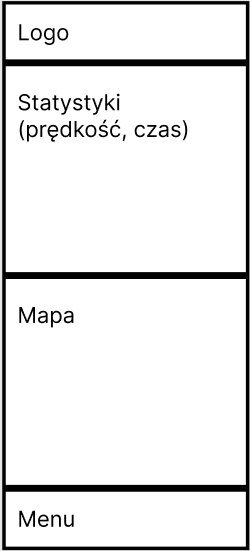
\includegraphics[width=.4\linewidth]{rys/ekran_treningu.png}
		\caption{Ekran treningu}
		\label{rys:rysunek001}
	\end{minipage}%
	\begin{minipage}{.5\textwidth}
		\centering
		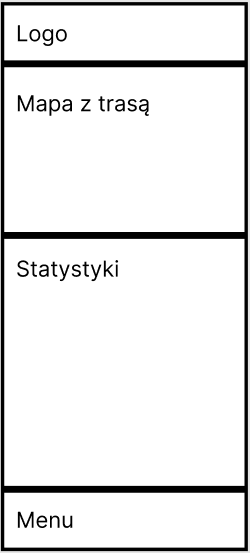
\includegraphics[width=.4\linewidth]{rys/ekran_podsumowania.png}
		\caption{Ekran podsumowania}
		\label{rys:rysunek002}
	\end{minipage}
\end{figure}

Ekran krokomierza Rys. \ref{rys:rysunek003} (s. \pageref{rys:rysunek003}) ma zawierać liczbę zrobionych w~bieżącym dniu kroków. Ekran krokomierza powinien być ekranem głównym, który użytkownik widzi po otwarciu aplikacji, ponieważ zawiera on, które prawdopodobnie są najbardziej interesujące w dany momencie. Oprócz tego w momencie rozpoczęcia treningu na tym ekranie ma~pojawić się dodatkowy licznik pokazujący tylko liczbę kroków zrobionych w trakcie treningu.

\begin{figure}[!htb]
	\centering
	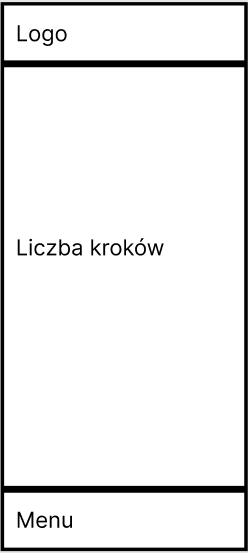
\includegraphics[width=.2\linewidth]{rys/ekran_krokomierza.png}
	\caption{Ekran krokomierza}
	\label{rys:rysunek003}
\end{figure}

Ekran zawierający historię odbytych treningów Rys. \ref{rys:rysunek005} (s. \pageref{rys:rysunek005}) powinien przedstawiać je w~postaci listy. Każdy wpis listy powinien zawierać datę treningu, a~po~naciśnięciu na dany wpis to ma się otworzyć ekran taki sam jak ekran podsumowania po zakończonym treningu, ale tym razem powiniem pokazywać zapisane dane z wybranego treningu. Ekran ustawień Rys. \ref{rys:rysunek006} (s. \pageref{rys:rysunek006}) też powinny być przedstawione w postaci listy. Kliknięcie w wybraną opcję ma otworzyć okienko wpisu zmiany wartości danej opcji.

\begin{figure}[!htb]
	\centering
	\begin{minipage}{.5\textwidth}
		\centering
		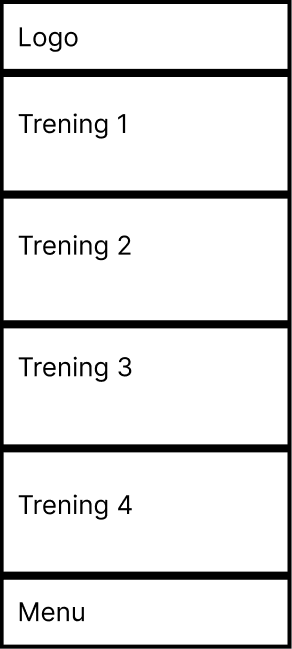
\includegraphics[width=.4\linewidth]{rys/ekran_historii.png}
		\caption{Ekran historii}
		\label{rys:rysunek005}
	\end{minipage}%
	\begin{minipage}{.5\textwidth}
		\centering
		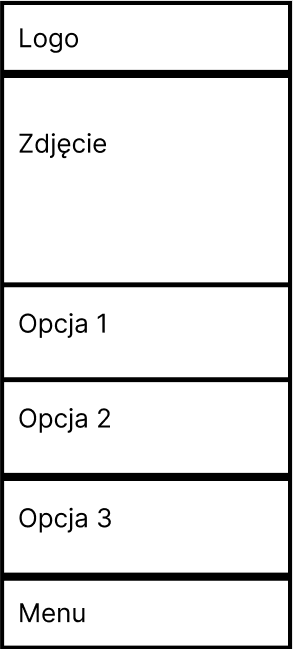
\includegraphics[width=.4\linewidth]{rys/ekran_ustawien.png}
		\caption{Ekran ustawień}
		\label{rys:rysunek006}
	\end{minipage}
\end{figure} 

Aby ułatwić użytkownikom nawigację po aplikacji, na dole ekranu powinno znajdować się intuicyjne menu, które pozwoli na szybkie przejście między poszczególnymi funkcjami. W menu tym powinny znaleźć się przyciski, które po kliknięciu przeniosą użytkownika do ekranu krokomierza, treningu, historii odbytych treningów oraz ekranu ustawień. Dzięki takiemu rozwiązaniu użytkownicy będą mogli łatwo i szybko dostępować do interesujących ich funkcji, co zwiększy komfort i efektywność korzystania z aplikacji.

Kolorystyka aplikacji powinna być starannie dobrana, aby zapewnić przyjemne i komfortowe doświadczenie użytkownikom. Optymalnym rozwiązaniem będzie zastosowanie odcieni zieleni, które są łagodne dla oczu i nie powodują dyskomfortu podczas dłuższej pracy z aplikacją. Dodatkowo, modernistyczny i nowoczesny wygląd aplikacji pozwoli użytkownikom poczuć, że korzystają z produktu wysokiej jakości, co zwiększy ich zadowolenie i satysfakcję z jej użytkowania. Dlatego ważne jest, aby projekt graficzny był przemyślany i dopracowany, aby spełniał wszystkie wymagania funkcjonalne i estetyczne.
   \newpage
\section{Określenie wymagań szczegółowych}		%2

\subsection{Środowisko programistyczne}  %2.1

\hspace{0.60cm}Aplikacja zostanie napisana korzystając z platformy Xamarin.Forms\footnote{Dokumentacja Xamarin.Forms   hhttps://learn.microsoft.com/en-us/xamarin/xamarin-forms/\cite{www6}.}. Jest to środowisko umożliwiające tworzenie aplikacji za pomocą języka XAML oraz kodu w~języku C\#.
Xamarin to platforma typu open source do tworzenia nowoczesnych i~wydajnych aplikacji dla systemów iOS, Android i Windows za pomocą platformy .NET. Xamarin to warstwa abstrakcji, która zarządza komunikacją udostępnionego kodu z~bazowym kodem platformy. Xamarin.Forms umożliwia deweloperom tworzenie aplikacji Xamarin.iOS, Xamarin.Android i Windows z pojedynczej udostępnionej bazy kodu. Xamarin.Forms Umożliwia deweloperom tworzenie interfejsów użytkownika w~języku XAML z użyciem kodu w języku C\#. Te interfejsy użytkownika są renderowane jako wydajne kontrolki natywne na każdej platformie. \\ Oto kilka przykładów funkcji udostępnianych przez Xamarin.Forms:

\begin{itemize}
	\item Język interfejsu użytkownika XAML,
	\item Powiązanie danych,
	\item Gestów,
	\item Efekty,
	\item Style
\end{itemize}

Dodatkowo, w celu koordynacji wykonywania projektu, organizacji kodu oraz ogólnego wspomagania pracy wykorzystany zostanie system kontroli wersji oprogramowania Git. Zapewnia on:

\begin{itemize}
	\item Dobre wsparcie dla rozgałęzionego procesu tworzenia oprogramowania: jest dostępnych kilka algorytmów łączenia zmian z dwóch gałęzi, a także możliwość dodawania własnych algorytmów,
	\item Każdy programista posiada własną kopię repozytorium, do której może zapisywać zmiany bez połączenia z siecią; następnie zmiany mogą być wymieniane między lokalnymi repozytoriami. Programista może także dodawać oraz usuwać gałęzie, 
	\item Efektywną pracę z dużymi projektami, jest o rzędy wielkości szybszy niż niektóre konkurencyjne rozwiązania
\end{itemize}

\subsection{Ogólny wygląd interfejsu}  %2.2

\hspace{0.60cm}Aplikacja będzie podzielona na podstrony. Na dole będzie znajdować się menu z opcjami. Wybór poszczególnej opcji w menu wyświetli daną podstronę w ekranie aplikacji. Kolejne podstrony to: Kroki, Trening, Historia, Ustawienia.

\subsection{Krokomierz}  %2.3

\hspace{0.60cm}W zakładce Kroki aplikacja będzie wyświetlała, korzystając z odpowiedniego sensora (krokomierza), liczbę kroków jaką użytkownik wykonał od rozpoczęcia treningu. Moduł krokomierza jest wymagany by zwiększyć wiarygodność aplikacji. Zastosowanie krokomierza umożliwia wykluczenie wpisów podejrzanych, które mogłyby wystąpić, gdyby użytkownik jechał na przykład rowerem lub samochodem. Takie rozwiązanie jest normalne w tego typu aplikacjach. Oprogramowanie Android w wersjach 4.4 i wyższych posiada wsparcie dla sensorów takich jak detektor kroków oraz licznik kroków. Kroki podczas biegu są łatwiejsze do odróżnienia od tych podczas zwykłego spaceru ze względu na bardziej wyraźne oddziaływanie na sensory. Tak więc jest duże prawdopodobieństwo, że krokomierz będzie bardzo dokładnie mierzył kroki, a~system będzie działał niezawodnie w wyjątkowych sytuacjach.

\subsection{Moduł GPS}  %2.4

\hspace{0.60cm}W zakładce Trening aplikacja będzie wyświetlała pomiar biegu użytkownika, a~dokładniej mówiąc pomiar przebiegniętego dystansu, prędkości biegu w danej chwili oraz czasu . Odbywa się to na podstawie informacji o jego pozycji. Można to zrealizować na kilka sposobów. Te sposoby to: wykorzystanie globalnego systemu pozycjonowania (GPS), technologia lokalizacji wieży komórkowej lub lokalizacja za pomocą WiFi Powinno się wybrać sposób najbardziej odpowiedni dla naszej aplikacji biorąc pod uwagę przede wszystkim środowisko w jakim będzie ona używana.

W naszym przypadku jest to system GPS, gdyż zapewnia on najdokładniejsze dane lokalizycyjne, wykorzystuje najwięcej mocy i działa najlepiej na zewnątrz, co~w~naszym przypadku jest kluczowe dla odpowiedniego działania aplikacji. Zakładając, że użytkownik przemieszcza się, można zdefiniować jego pozycję z dokładnością od około 6 do 100 metrów.

Aplikacja z obsługą lokalizacji wymaga dostępu do czujników sprzętowych urządzenia w celu odbierania danych GPS. Dostęp jest kontrolowany za pomocą odpowiednich uprawnień w manifeście Androida aplikacji (plik AndroidManifest.xml). \\ Dostępne są dwa uprawnienia: \\ \textit{ACCESS\_COARSE\_LOCATION} - zapewnia aplikacji dostęp do dostawcy GPS oraz \textit{ACCESS\_FINE\_LOCATION} - umożliwia aplikacji dostęp do sieci komórkowej i~WiFi lokalizacji. Wymagane dla dostawcy sieci gdy ACCESS\_COARSE\_LOCATION jest nieustawiony.

\subsection{Mapy Google}  %2.5

\hspace{0.60cm}W zakładce Trening będzie wyświetlana również, korzystając z modułu GPS, aktualna pozycja użytkownika na Mapach Google. Dostęp do Map Google jest możliwy dzięki API (Maps SDK for Android) udostępnianego przez Google. Dostęp do~tego API jest uzyskiwany z kluczem API, który został wygenerowany w panelu Google Cloud API. Możliwość wyświetlania pobranej mapy w aplikacji jest możliwa korzystając z pakietu NuGet Xamarin.Forms.Maps\footnote{Dokumentacja na stronie   https://learn.microsoft.com/en-us/xamarin/xamarin-forms/user-interface/map/setup\cite{www3}.}. Na mapie będzie także rysowana linią (klasa Polyline z wyżej wymienionego pakietu) trasa przebyta w trakcie treningu. 

\subsection{Baza danych SQLite} %2.6

\hspace{0.60cm}SQLite to mała, szybka i przystosowana do osadzania baza danych SQL oparta na systemie plików typu open source. Nie posiada oddzielnego komponentu serwerowego, jak tradycyjne bazy danych. Jest ona darmowa i zawiera wszystko co~najważniejsze w relacyjnej bazie danych. Jest ona najczęściej instalowana na serwerach. Pozwala zgrabnie zarządzać użytkownikami i świetnie nadaje się do małych oraz średniej wielkości projektów. Znajduje się w dokładnie jednym pliku. Bardzo często wybierana jako baza dla aplikacji iOS oraz Android. Wspiera SQL. Sprawdza się na urządzeniach z ograniczoną możliwościami instalacji dodatkowego oprogramowania, takimi jak smartfony, dekodery i telewizory. Również jest świetnym silnikiem bazodanowym dla witryn o niskim i średnim ruchu. Przy odpowiedniej konfiguracji jest wydajny i może pełnić rolę zarówno silnika do analizy dużego zbioru informacji jak i cache serwer dla danych z częstym odczytem.



   	\newpage
\section{Projektowanie}		%3
%Opis przygotowania narzędzi (git, visual studio). Wybór i opis bibliotek, klas. Szkic layoutów. Pseudo kody. Opisy wykorzystanych algorytmów (np. algorytm sortowania). Dokładniejsze określenie założeń i działania aplikacji, (np.: ten przycisk otworzy takie okno a w tym oknie wpisujemy takie dane).

\subsection{Przygotowanie narzędzi (Git, Visual Studio)}		%3.1

\subsubsection{Visual Studio} %3.1.1
\hspace{0.60cm}Pierwszym i oczywistym krokiem, który musimy wykonać jest przygotowanie właściwych technologii i środowisk, które posłużą do tworzenia naszego projektu. Jako środowisko programistyczne wybrano Visual Studio 2022 i dostępną na nim wspomnianą wcześniej platformę Xamarin.Forms. W celu instalacji tego narzędzia, pobieramy plik instalacyjny ze strony Microsoftu\footnote{Plik instalacyjny na stronie  https://visualstudio.microsoft.com/pl/vs\cite{www1}.}. Podczas instalacji, w menedżerze dodatkowych pakietów, wybieramy pakiet \textit{Mobile developement with .NET}, zaznaczając też opcjonalne dodatki w zależności od wymagań (np. Xamarin, emulator Androida itd.). Środowisko Visual Studio posiada zintegrowany system kontroli wersji oprogramowania Git, który będzie wspomagał naszą pracę. 

\subsubsection{Git} %3.1.2
Na stronie Github stworzone zostało zdalne repozytorium, do którego wysyłane będą kolejne wersje naszego projektu, z możliwością kontrybucji ze strony członków zespołu programistów. Lokalnie, na maszynach programistów zainstalowano dodatkowe narzędzie jakim jest desktopowa aplikacja Git for Windows, która dostarcza emulację BASH wykorzystywaną do uruchamiania Git'a z wiersza poleceń. Jest to duże udogodnienie dla osób, które czują się pewniej pracując z terminalem systemu Linux. Plik instalacyjny można pobrać ze strony\footnote{Plik instalacyjny na stronie https://git-scm.com/download/win\cite{www2}.}.

\subsection{Szkice layoutów}		%3.2

\subsubsection{Zakładka Kroki} %3.2.1

\hspace{0.60cm}W zakładce Kroki rys. \ref{rys:rysunek001a} (s. \pageref{rys:rysunek001a}) użytkownik ma możliwość rozpoczęcia liczenia wykonanych kroków.

\begin{figure}[!htb]
	\centering
	
\includegraphics[width=.2\linewidth]{rys/kroki.png}
	\caption{Layout krokomierza}
	\label{rys:rysunek001a}
\end{figure}

Liczenie kroków wykonuje się przy wykorzystaniu modułu akcelerometra..

\subsubsection{Zakładka Trening} %3.2.2

\hspace{0.60cm}W zakładce Trening rys. \ref{rys:rysunek001b} (s. \pageref{rys:rysunek001b}) użytkownik ma możliwość rozpoczęcia treningu. Zaczyna się odliczanie i wyświetlanie na ekranie bieżącego czasu odbywanego treningu, pokonany dystans w metrach, bieżąca prędkość oraz teoretyczna ilość spalonych kalorii. Na środkowej części ekranu wyświetlana zostaje, przy wykorzystaniu modułów GPS oraz  Map Google bieżąca lokalizacja użytkownika. Za pomocą polilinii rysowana jest trasa, którą udaje się użytkownik. 

\begin{figure}[!htb]
	\centering
	\begin{minipage}{.5\textwidth}
		\centering
		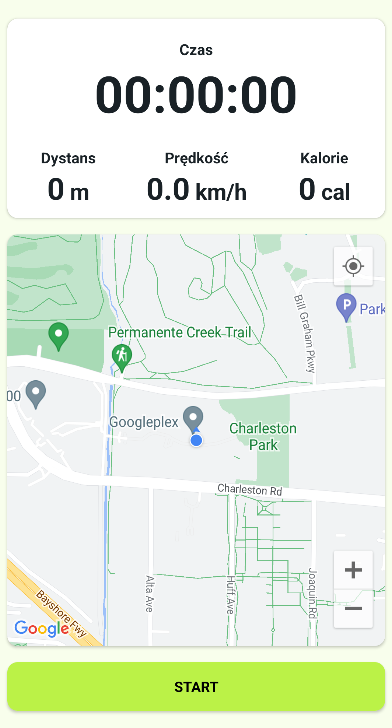
\includegraphics[width=.4\linewidth]{rys/trening.png}
		\caption{Layout treningu}
		\label{rys:rysunek001b}
	\end{minipage}%
	\begin{minipage}{.5\textwidth}
		\centering
		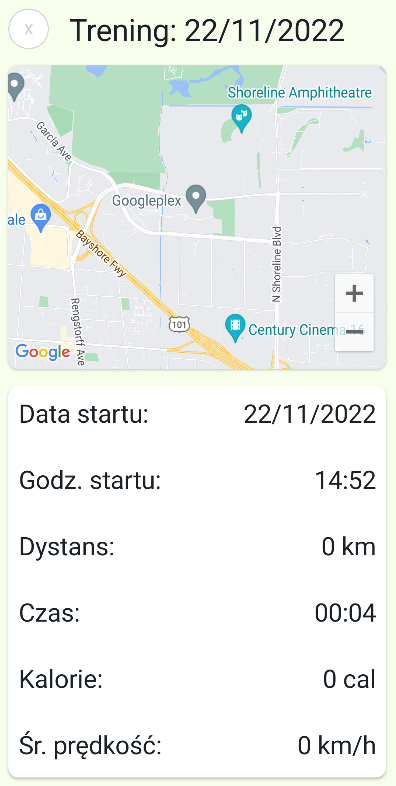
\includegraphics[width=.4\linewidth]{rys/trening2.png}
		\caption{Ekran podsumowania}
		\label{rys:rysunek001c}
	\end{minipage}
\end{figure}

Po zakończeniu treningu, w tej samej zakładce, wyświetlony zostaje ekran zawierający podsumowanie odbytego treningu. Jak pokazano na rys. \ref{rys:rysunek001c} (s. \pageref{rys:rysunek001c}), podsumowanie zawiera datę i czas rozpoczęcia treningu, przebyty dystans, czas treningu, spalone kalorie oraz średnią prędkość z jaką poruszał się użytkownik. 

\subsubsection{Zakładka Historia} %3.2.3

\hspace{0.60cm}W zakładce Historia, po zakończeniu kolejnych treningów, do bazy danych zapisywane są rekordy zawierające dane dotyczące odbytych w przeszłości treningów wraz z podstawywymi danymi jak data, czas oraz statystyki, co pokazano na rys. \ref{rys:rysunek001d} (s. \pageref{rys:rysunek001d}). Dane po zakończeniu treningu są najpierw zapisywane do bazy danych SQLite, następnie wyświetlane w zakładce Historia od najnowszego do najstarszego.

\begin{figure}[!htb]
	\centering
	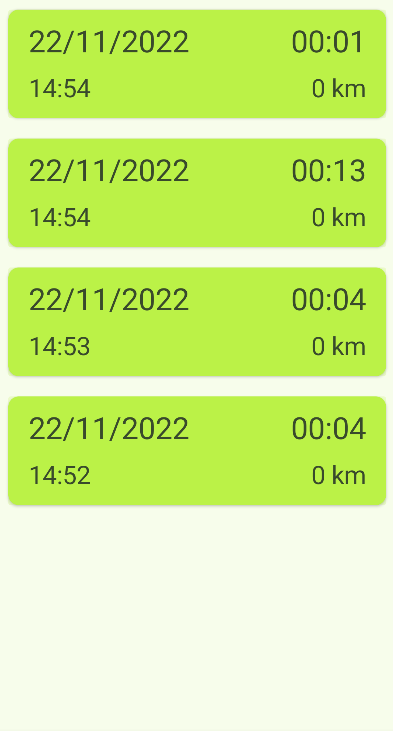
\includegraphics[width=.2\linewidth]{rys/historia.png}
	\caption{Layout historii treningów}
	\label{rys:rysunek001d}
\end{figure}

Wykorzystana w nim zostaje odpowiednia funkcja otwierająca widok statystyk i podsumowania.

\subsubsection{Zakładka Ustawienia} %3.2.4

\hspace{0.60cm}W zakładce Ustawienia rys. \ref{rys:rysunek001e} (s. \pageref{rys:rysunek001e}) użytkownik ma możliwość konfiguracji własnego konta użytkownika, swoich danych fizycznych oraz wieku, na podstawie których obliczane zostają statystyki traningu jak np. spalone kalorie. 

\begin{figure}[!htb]
	\centering
	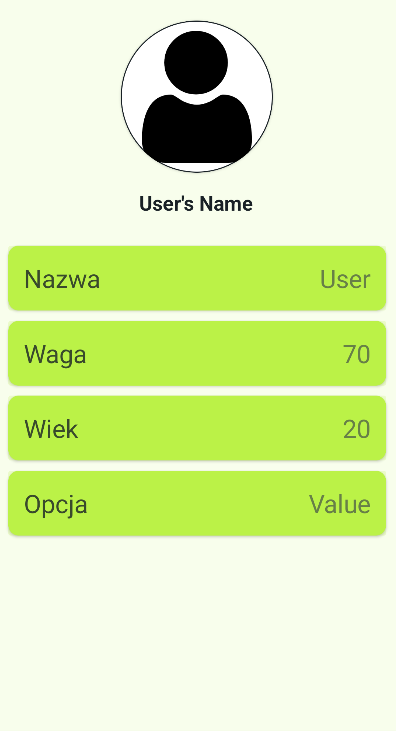
\includegraphics[width=.2\linewidth]{rys/ustawienia.png}
	\caption{Layout ustawień i opcji}
	\label{rys:rysunek001e}
\end{figure}
   	\newpage
\section{Implementacja}		%4
%Wkleić szkielet kodu, wraz z komentarzami. Opisać zmienne, struktury do czego służą. Opisać procedury, metody co wykonują. Opisać nowe zdefiniowane klasy. Opisać dziedziczenie. Opisać nowo utworzone pliki za co odpowiadają.

\subsection{Wybrane kody z objaśnieniami działania}		%4.1

\subsubsection{Zakładka Historia} %4.1.1

\hspace{0.60cm}Kod \ref{lst:listing-cpp} przedstawia sposób inicjalizacji połączenia z bazą danych SQLite:
\begin{lstlisting}[caption=Połączenie z bazą danych, label={lst:listing-cpp}, language=C++]
	public History()
	{
		InitializeComponent();
		
		_database = new SQLiteAsyncConnection(Path.Combine(Environment.
		GetFolderPath(Environment.SpecialFolder.LocalApplication
		Data), "trainingHistory.db3"));
	}
\end{lstlisting}

Kod \ref{lst:listing-cpp2} przedstawia sposób wypisania danych na ekran:
\begin{lstlisting}[caption=Wypisanie danych na ekran, label={lst:listing-cpp2}, language=C++]
	protected override async void OnAppearing()
	{
		base.OnAppearing();
		
		//Wypisanie danych na ekran
		collectionView.ItemsSource = await GetTrainingData();
	}
\end{lstlisting}

Kod \ref{lst:listing-cpp3} przedstawia sposóB w jaki pobierane są dane z bazy danych:
\begin{lstlisting}[caption=Pobranie danych z bazy, label={lst:listing-cpp3}, language=C++]
	public async Task<List<TrainingData>> GetTrainingData()
	{
		var query = await _database.Table<TrainingData>().ToListAsync();
		results = Enumerable.Reverse(query).ToList();
		return results;
	}
\end{lstlisting}

Kod \ref{lst:listing-cpp4} zawiera funkcję otwieracjącą widok statystyk i podsumowania:
\begin{lstlisting}[caption=Otwieranie widoku statystyk i podsumowania, label={lst:listing-cpp4}, language=C++]
	private async void OpenStatistics(object sender, EventArgs e)
	{
		var btn = (Button)sender;
		await Navigation.PushAsync(new StatisticsView(btn.ClassId));
	}
\end{lstlisting}

Kod \ref{lst:listing-cpp5} przedstawia sposób w jaki dane z bazy danych zostaną wypisane na ekran:
\begin{lstlisting}[caption=Wypisanie danych z bazy danych na ekran, label={lst:listing-cpp5}, language=C++]
	public async Task<List<TrainingData>> GetTrainingData()
	{
		var query = _database.Table<TrainingData>().Where(p => p.Id == buttonId);
		var result =  await query.ToListAsync();
		nazwa.Text = "Trening: " + result[0].DateDay;
		
		_databaseTraining = new SQLiteAsyncConnection(Path.Combine(Environment.GetFolderPath(Environment.SpecialFolder.LocalApplicationData), result[0].TrainingDatabase));
		var locations = await _databaseTraining.Table<CurrentData>().ToListAsync();
		
		Polyline polyline = new Polyline();
		polyline.StrokeColor = Color.FromHex("#192126");
		polyline.StrokeWidth = 20;
		foreach (var pos in locations)
		polyline.Geopath.Add(new Position(pos.Latitude, pos.Longitude));
		map.MapElements.Add(polyline);
		
		Position startPos = new Position(locations[0].Latitude, locations[0].Longitude);
		map.MoveToRegion(MapSpan.FromCenterAndRadius(startPos, Distance.FromKilometers(1)));
		
		
		dataStartu.Text = result[0].DateDay;
		godzinaStartu.Text = result[0].DateTime;
		dystans.Text = result[0].Distance;
		czas.Text = result[0].Time;
		calories.Text = result[0].Calories.ToString() + " cal";
		avrSpeed.Text = result[0].AvrSpeed.ToString() + " km/h";
		return result;
	}
\end{lstlisting}

\subsubsection{Zakładka Trening} %4.1.2

\hspace{0.60cm}Kod \ref{lst:listing-cpp6} przedstawia sposób inicjalizacji połączenia z bazą danych:
\begin{lstlisting}[caption=Połączenie z bazą danych, label={lst:listing-cpp6}, language=C++]
	public Training()
	{
		InitializeComponent();
		
		_database = new SQLiteAsyncConnection(Path.Combine(Environment.
		GetFolderPath(Environment.SpecialFolder.
		LocalApplicationData), "trainingHistory.db3"));
		_database.CreateTableAsync<TrainingData>();
		GetLocation();
	}
\end{lstlisting}

Kod \ref{lst:listing-cpp7} zawiera funkcję pobierająca lokalizację:
\begin{lstlisting}[caption=Pobranie lokalizacji, label={lst:listing-cpp7}, language=C++]
	private async void GetLocation()
	{
		//pobranie lokalizacji
		var request = new GeolocationRequest(GeolocationAccuracy.Best);
		var location = await Geolocation.GetLocationAsync(request);
		
		if (location != null)
		{
			position = new Position(location.Latitude, location.Longitude);
			
			//przesuniecie widoku na lokalizacje przeciwnika
			map.MoveToRegion(MapSpan.FromCenterAndRadius(position, Distance.
			FromKilometers(0.5)));
			
			if (isTraining)
			{   
				//zapis danych lokalizacji
				positionsList.Add(new PositionList { Location = location, TimeLasted = 
					(hours * 3600 + mins * 60 + secs) });
				await SaveCurrentData(new CurrentData
				{
					Latitude = location.Latitude,
					Longitude = location.Longitude,
					TimeLasted = (hours * 3600 + mins * 60 + secs)
				});
				UpdateInfo();
			}
			
		}
		
		//pobranie lokalizacji wywolywane co 2 sekundy
		await Task.Delay(2000);
		GetLocation();
		
	}
\end{lstlisting}

Kod \ref{lst:listing-cpp8} wprowadza możliwość rozpoczęcia treningu:
\begin{lstlisting}[caption=Rozpoczęcie treningu, label={lst:listing-cpp8}, language=C++]
	private void StartTraining(object sender, EventArgs e)
	{
		btnStartF.IsVisible = false;
		btnResumeF.IsVisible = false;
		btnEndF.IsVisible = false;
		btnStopF.IsVisible = true;
		isTraining = true;
		startDate = DateTime.Now;
		
		//baza danych lokalizacji w treningu
		_databaseTraining = new SQLiteAsyncConnection(Path.Combine(Environment.GetFolderPath(Environment.SpecialFolder.LocalApplicationData), "training" + startDate.ToString("dd_MM_yyyy_HH_mm_ss") + ".db3"));
		_databaseTraining.CreateTableAsync<CurrentData>();
		
		//inicjalizacja timera
		timer = new Timer();
		timer.Interval = 1000;
		timer.Elapsed += Timer_Elapsed;
		timer.Start();
	}
\end{lstlisting}

Kod \ref{lst:listing-cpp9} zawiera funkcję liczącą sekundy, wywoływaną co sekundę:
\begin{lstlisting}[caption=Liczenie sekund (co sekundę:), label={lst:listing-cpp9}, language=C++]
	private void Timer_Elapsed(object sender, ElapsedEventArgs e)
	{
		secs++;
		if (secs == 59)
		{
			mins++;
			secs = 0;
		}
		if (mins == 59)
		{
			hours++;
			mins = 0;
		}
		Device.BeginInvokeOnMainThread(() =>
		{
			timerValue.Text = string.Format("{0:00}:{1:00}:{2:00}", hours, mins, secs);
		});
	}
\end{lstlisting}

Kod \ref{lst:listing-cpp10} umożliwia zakończenie treningu oraz obsługę danych po odbytym treningu:
\begin{lstlisting}[caption=Zakończenie treningu\, zapis danych do bazy i ich podsumowanie, label={lst:listing-cpp10}, language=C++]
	private async void EndTraining(object sender, EventArgs e)
	{
		btnResumeF.IsVisible = false;
		btnEndF.IsVisible = false;
		btnStopF.IsVisible = false;
		btnStartF.IsVisible = true;
		
		//zapis danych treningu do glownej bazy danych
		await SaveTrainingData(new TrainingData
		{
			DateDay = startDate.ToString("dd/MM/yyyy"),
			DateTime = startDate.ToString("HH:mm"),
			Time = string.Format("{0:00}:{1:00}", (hours * 60 + mins), secs),
			Distance = way.ToString() + " km",
			Calories = caloriesBurned,
			AvrSpeed = avrSpeed, 
			TrainingDatabase = "training" + startDate.ToString("dd_MM_yyyy_HH_mm_ss") + ".db3"
		});
		
		//otwarcie strony podsumowania treningu
		await Navigation.PushAsync(new StatisticsView(CountTrainings().Result.ToString()));
		
		//wyzerowanie zmiennych pomiarowych
		way = 0;
		tempo = 0;
		caloriesBurned = 0;
		avrSpeed = 0;
		speedSum = 0;
		timerValue.Text = "00:00:00";
		amountDistance.Text = "0";
		amountCalories.Text = "0";
		amountSpeed.Text = "0.0";
		hours = 0;
		mins = 0;
		secs = 0;
		map.MapElements.Clear();
	}
\end{lstlisting}

Kod \ref{lst:listing-cpp11} zawiera funkcję aktualizującą informacje na ekranie:
\begin{lstlisting}[caption=Aktualizowanie informacji na ekranie, label={lst:listing-cpp11}, language=C++]
	 private void UpdateInfo()
	{
		//polyline rysuje trase na mapie
		Polyline polyline = new Polyline();
		polyline.StrokeColor = Color.FromHex("#192126");
		polyline.StrokeWidth = 20;
		int length = positionsList.Count - 1;
		double tmpWay;
		if (length > 1)
		{
			//ustawienie lini na dwie ostanie pozycje
			polyline.Geopath.Add(new Position(positionsList[length - 1].Location.Latitude, positionsList[length - 1].Location.Longitude));
			polyline.Geopath.Add(new Position(positionsList[length].Location.Latitude, positionsList[length].Location.Longitude));
			//wywolanie linii na mapie
			map.MapElements.Add(polyline);
			
			//obliczenia parametrow treningu
			tmpWay = Location.CalculateDistance(positionsList[length].Location, positionsList[length - 1].Location, DistanceUnits.Kilometers);
			way = Math.Round((way + tmpWay), 3);
			tempo = (tmpWay / (positionsList[length].TimeLasted - positionsList[length - 1].TimeLasted)) * 3600;
			tempo = Math.Round(tempo, 1);
			speedSum += tempo * (positionsList[length].TimeLasted - positionsList[length - 1].TimeLasted);
			avrSpeed = speedSum / (positionsList[length].TimeLasted);
			avrSpeed = Math.Round(avrSpeed, 1);
			//kalorie na minute = (MET * 3.5 * waga) / 200
			//MET - ile razy wiecej kalorii spala przy danej aktywnosci w porowaniu do odpoczynku
			caloriesBurned = ((avrSpeed * 3.5 * weight) / 200) * (((double)positionsList[length].TimeLasted) / 60);
			caloriesBurned = Math.Round(caloriesBurned, 1);
		}
		
		//wyswietlenie dystansu w okreslonym formacie zaleznym od dystansu
		if (way < 1)
		{
			amountDistance.Text = (way * 1000).ToString();
			distanceSize.Text = " m";
		}
		else if (way < 10)
		{
			amountDistance.Text = string.Format("{0:0.00}", way);
			distanceSize.Text = " km";
		}
		else if (way < 100)
		{
			amountDistance.Text = string.Format("{0:00.0}", way);
			distanceSize.Text = " km";
		}
		else
		{
			amountDistance.Text = string.Format("{0:000}", way);
			distanceSize.Text = " km";
		}
		
		//wyswietlenie predkosci w okreslonym formacie
		if (tempo < 10)
		amountSpeed.Text = string.Format("{0:0.0}", tempo);
		else
		amountSpeed.Text = string.Format("{0:00}", tempo);
		//wyswietlenie spalonych kalorii
		if (caloriesBurned < 10)
		amountCalories.Text = caloriesBurned.ToString();
		else
		amountCalories.Text = string.Format("{0:00}", caloriesBurned);
	}
\end{lstlisting}

Kod \ref{lst:listing-cpp12} wykonuje zapis danych treningu do bazy danych:
\begin{lstlisting}[caption=Zapis danych do bazy danych, label={lst:listing-cpp12}, language=C++]
	public Task<int> SaveTrainingData(TrainingData trainingData)      
	{
		return _database.InsertAsync(trainingData);
	}
\end{lstlisting}

\subsubsection{Zakładka Kroki} %4.1.2

Kod \ref{lst:listing-cpp13} implementuje modułu Step\_Counter, wykorzystujący czujnik akcelerometr:
\begin{lstlisting}[caption=Krakomierz i akcelerometr, label={lst:listing-cpp13}, language=C++]
	public partial class StepCounter : ContentPage
	{
		//inicjalizacja listy przechowujacej liczbe krokow
		List<double> accData = new List<double>();
		int stepsNumber = 0;
		DateTime czas = DateTime.Now;
		TimeSpan interval = TimeSpan.FromSeconds(0.1);
		
		
		public StepCounter()
		{
			InitializeComponent();
			
			Accelerometer.ReadingChanged += Accelerometer_ReadingChanged;
		}
		
		//implementacja modulu akcelerometra
		void Accelerometer_ReadingChanged(object sender, AccelerometerChangedEventArgs args)
		{
			if (DateTime.Now - czas > interval)
			{
				czas = DateTime.Now;
				var xVal = args.Reading.Acceleration.X * 10;
				var yVal = args.Reading.Acceleration.Y * 10;
				var zVal = args.Reading.Acceleration.Z * 10;
				var accValue = Math.Sqrt(xVal * xVal + yVal * yVal + zVal * zVal) - 10;
				if (accData.Count > 240)
				accData.RemoveAt(0);
				accData.Add(accValue);
				
				//petla liczaca kroki
				if (accData.Count > 1)
				{
					for (int i = 1; i < accData.Count - 1; i++)
					{
						if (accData[i] > 1)
						{
							if (accData[i] > accData[i - 1] && accData[i] > accData[i + 1])
							{
								stepsNumber++;
								accData.Clear();
							}
						}
						
					}
				}
				amountSteps.Text = stepsNumber.ToString();
			}
		}
\end{lstlisting}

Kod \ref{lst:listing-cpp14} zawiera funkcję dającą możliwość rozpoczęcia i zakończenia liczenia kroków:
\begin{lstlisting}[caption=Rozpoczęcia i zakończenie liczenia kroków, label={lst:listing-cpp14}, language=C++]
	void Button_Cliked(object sender, EventArgs e) 
	{
		try
		{
			if (Accelerometer.IsMonitoring)
			{
				Accelerometer.Stop();
				btn.Text = "Start";
			}   
			else
			{
				Accelerometer.Start(SensorSpeed.UI);
				btn.Text = "Stop";
			}
			
		}
		catch (FeatureNotSupportedException fnsEx)
		{
			// Not supported on device
		}
		catch (Exception ex)
		{
			// Something else went wrong
		}
	}
\end{lstlisting}
   	\newpage
\section{Testowanie}	%5
%Opisujemy testy, sprawdzamy czy nie generuje błędów.



   	\newpage
\section{Podręcznik użytkownika}  %6
%Opis jak używać programu. Mogą być z zrzut ekranu razem z opisem. 



       
%%%%%%%%%%%%%%%%%%% koniec treść główna dokumentu %%%%%%%%%%%%%%%%%%%%%
	\newpage
    \addcontentsline{toc}{section}{Literatura}  
	\printbibliography

    \newpage
    \hypersetup{linkcolor=black}
    \renewcommand{\cftparskip}{3pt}
    \clearpage
    \renewcommand{\cftloftitlefont}{\Large\bfseries\sffamily}
    \listoffigures
    \addcontentsline{toc}{section}{Spis rysunków}
	\thispagestyle{fancy}
	
    \newpage
    \renewcommand{\cftlottitlefont}{\Large\bfseries\sffamily}
    \def\listtablename{Spis tabel}
    \addcontentsline{toc}{section}{Spis tabel}\listoftables 
	\thispagestyle{fancy}
	
	\newpage
	\renewcommand{\cftlottitlefont}{\Large\bfseries\sffamily}
	\renewcommand\lstlistlistingname{Spis listingów}
	\addcontentsline{toc}{section}{Spis listingów}\lstlistoflistings 
	\thispagestyle{fancy}
	


    %lista rzeczy do zrobienia: wypisuje na koñcu dokumentu, patrz: pakiet todo.sty
    \todos
    %koniec listy rzeczy do zrobienia
\end{document}
